\documentclass[aspectratio=169]{beamer}
\usetheme{Madrid}
\usepackage[utf8]{inputenc}
\usepackage[T1]{fontenc}
\usepackage{tikz}
\usepackage{amssymb}
\usepackage{graphicx}
\setbeamertemplate{navigation symbols}{}
\setbeamercolor{title}{fg=white,bg=blue!70!cyan}
\setbeamercolor{frametitle}{fg=white,bg=blue!70!cyan}
\setbeamercolor{block title}{bg=blue!70!cyan!20,fg=black}
\setbeamercolor{block body}{bg=blue!70!cyan!8,fg=black}
\setbeamercolor{item}{fg=blue!70!cyan}
\setbeamercolor{itemize item}{fg=blue!70!cyan}
\setbeamertemplate{itemize item}[triangle]

\title{G10 — Design \& Capstone}
\subtitle{Plan → build → test → ship YOUR game}
\author{ByteForge --- Grade 7 --- Game Maker}
\date{}

\begin{document}

\begin{frame}
    \titlepage
\end{frame}

\begin{frame}{Today's Plan}
    \begin{itemize}
        \item Design Your Game
        \item Score \& Win Screen
        \item[$\bigstar$] BOSS --- Ship Your Own Game
    \end{itemize}
\end{frame}

\begin{frame}{Planning BEFORE building}
    \large
    \begin{itemize}
        \item A clear, checkable win condition ("reach 20 points") is easier to build AND test than a vague goal like "make it fun".
    \end{itemize}
\end{frame}


\begin{frame}{Live, updating feedback for the player}
    \large
    \begin{itemize}
        \item Redrawing the score every frame means you never have to manually "update" the display
        \item It always reflects the current value.
    \end{itemize}
\end{frame}


\begin{frame}{FINAL BOSS — everything from the whole year}
    \large
    \begin{itemize}
        \item A state machine, player input, a win condition, and at least one function you define
        \item Every major idea, combined into a game YOU designed.
    \end{itemize}

    \begin{center}
    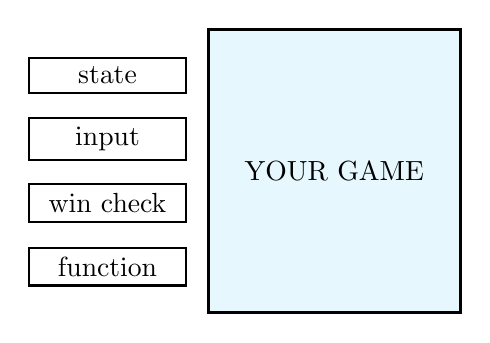
\begin{tikzpicture}[scale=0.9]

        \node[draw, thick, minimum width=2cm] at (0,0.9) {state};
        \node[draw, thick, minimum width=2cm] at (0,0) {input};
        \node[draw, thick, minimum width=2cm] at (0,-0.9) {win check};
        \node[draw, thick, minimum width=2cm] at (0,-1.8) {function};
        \node[draw, very thick, minimum width=3.2cm, minimum height=3.6cm, fill=cyan!10] at (3.2,-0.45) {YOUR GAME};
    \end{tikzpicture}
    \end{center}
\end{frame}


\begin{frame}{Playtest, then iterate}
    \large
    \begin{itemize}
        \item Real developers ALWAYS playtest and adjust at least once
        \item A first draft is rarely the final version.
    \end{itemize}
\end{frame}

\begin{frame}{Real-World Examples}
    \large
    \begin{itemize}
        \item Every shipped game went through exactly this: a design document, a build, a playtest, then changes based on what real players actually did
        \item Not what the designer assumed they'd do. Minecraft itself is still playtested and balanced this way every update (mob health, drop rates, tool durability all get tuned from real player data).
    \end{itemize}
\end{frame}


\begin{frame}{Let Them Discover}
    \Large
    Before opening the platform: sketch your game idea on paper — one sentence for "how do you win", and one sketch of what the screen looks like. Trade with a partner and ask: is the win condition actually checkable?
\end{frame}

\begin{frame}{Your Turn}
    \Large
    Open the student map, find \textbf{G10 — Design \& Capstone}, and work through it
    hands-on --- everything you just saw, they now do themselves.
\end{frame}

\end{document}
